%!TEX root = ../username.tex
\chapter{Mathematics In Music} \label{mathinmusic}

\section{The Harmonic Series} \label{mathinmusic:harmonic}

An important concept for pitch sounds is the harmonic series.
Pitched sounds have a \textit{fundamental frequency} from which an overtone series is produced.
\textit{Overtones} are any frequencies higher than the fundamental frequency.
The \textit{harmonic series}\footnote{Note that this harmonic series is different from, though related to, the mathematical harmonic series.} is a restricted subset of the overtone series consisting of the integer multiples of the fundamental frequency.
For example, consider the open A string of a cello which is pitched as an A3.
In other words it has a fundamental frequency of $220$ Hz.
Doubling this frequency gives $440$ Hz, or an octave above the fundamental frequency.
Tripling the frequency gives $660$ Hz, which is an E5.
This continues, so multiplying by $4$ gives a frequency two octaves above the fundamental, multiplying by $5$ produces a C$\sharp$6, multiplying by $6$ gives an E6, multiplying by $7$ gives a G6, and multiplying by $8$ gives an A6, three octaves above the fundamental frequency.
We could go on, and eventually the frequencies would pass out of the human hearing range (approximately $20000$ Hz).

The presence of the overtone series, and in particular the harmonic series is what makes a sound pitched.
See Figures \ref{fig:sin}, \ref{fig:harmonics}, and \ref{fig:summedHarmonics} for examples of a sine wave, the first five harmonic sine waves overlayed on top of each other, and the sum of the first five harmonics, respectively.
Percussive sounds such as hitting a drum or dropping a brick do produce pressure in the air, but the oscillations of the pressure are not regular, and so do not produce any pitched frequencies.

\begin{figure}
	\centering
	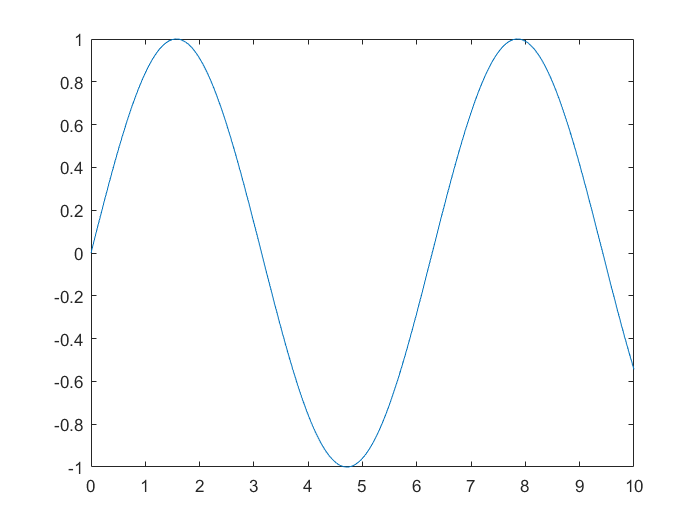
\includegraphics[width=\textwidth]{../figures/sinWave.png}
	\caption{A pure sine wave}
	\label{fig:sin}
\end{figure}

\begin{figure}
	\centering
	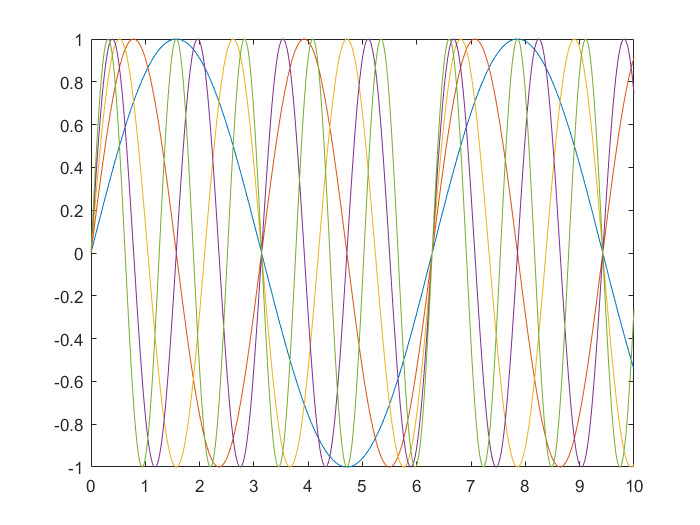
\includegraphics[width=\textwidth]{../figures/harmonicSinWaves.png}
	\caption{The first five harmonic frequencies of a sine wave.}
	\label{fig:harmonics}
\end{figure}

\begin{figure}
	\centering
	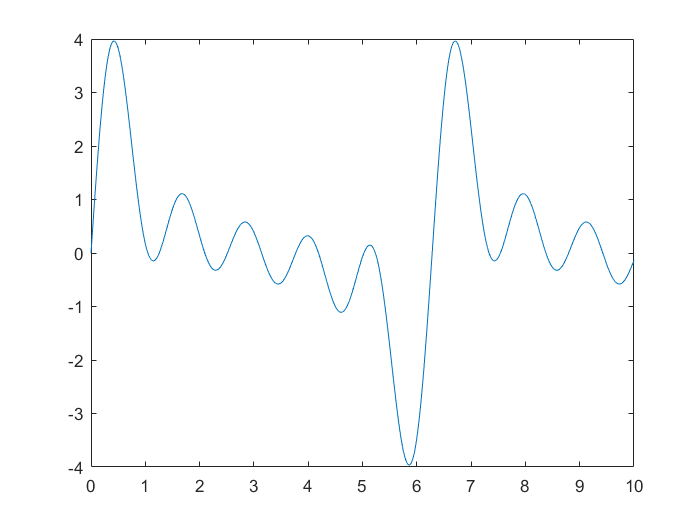
\includegraphics[width=\textwidth]{../figures/summedSinWaves.png}
	\caption{The sum of the first five harmonic sine waves.}
	\label{fig:summedHarmonics}
\end{figure}

Brass instruments are built with the harmonic series in mind.
For example, the tenor trombone has a fundamental pitch of a B$\flat$1, or $58.87$ Hz.
The pitches that can be played on the instrument in first position (i.e. without moving the slide, which would change the fundamental frequency) are those of the harmonic series based on B$\flat$1.
Thus the trombone can theoretically play B$\flat$1, B$\flat$2, F3, B$\flat$3, D4, F4, a very flat G$\sharp$4, B$\flat$4, C5, D5, a very flat E5, F5, and so on.
In practice however, due to the physical demands of the player, any note above B$\flat$4 is uncommon, and any note above D5 is rare.

When discussing brass instruments, there are some modifications made to the frequencies by the shapes of the the bell and mouthpiece of the instrument, but those are beyond the scope of this project.

% Gabriel's Horn

\section{Intervals Between Notes} \label{mathinmusic:intervals}

In order to discuss intervals between notes, we must first choose a tuning system.
The two most common tuning systems are just intonation and equal temperament.

\subsection{Just Intonation} \label{mathinmusic:intervals:just}

Just intonation is based on the concept of perfect intonation, whereby an interval is defined as multiplying a pitch be some rational constant.
Table \ref{table:justintervals} contains the rational ratios for intervals through the first octave.

\begin{table}
	\centering
	\begin{tabular}{c c c}
		Semitones From Base & Ratio & Interval Name\\
		\hline
		0 & $\frac{1}{1}$ & unison\\[4pt]
		1 & $\frac{16}{15}$ & minor second\\[4pt]
		2 & $\frac{9}{8}$ & major second\\[4pt]
		3 & $\frac{6}{5}$ & minor third\\[4pt]
		4 & $\frac{5}{4}$ & major third\\[4pt]
		5 & $\frac{4}{3}$ & perfect fourth\\[4pt]
		6 & $\frac{45}{32}$ & diminished fifth/tritone\\[4pt]
		7 & $\frac{3}{2}$ & perfect fifth\\[4pt]
		8 & $\frac{8}{5}$ & minor sixth\\[4pt]
		9 & $\frac{5}{3}$ & major sixth\\[4pt]
		10 & $\frac{9}{5}$ & minor seventh\\[4pt]
		11 & $\frac{15}{8}$ & major seventh\\[4pt]
		12 & $\frac{2}{1}$ & octave
	\end{tabular}
	\caption{Ratios for intervals under just intonation.}
	\label{table:justintervals}
\end{table}

The just tuning system produces the best sounding intervals and is used to tune intervals by ear.
The downside is that the size of an interval is different than the sum of semi tones to reach the same interval.
For example, the frequency of major third above a given note is $\frac{6}{5}$ that of the given note.
Building that same interval (4 semi tones) by moving up the chromatic scale, however, the ratio is $(\frac{16}{15})^{4} = \frac{65536}{50625} \approx \frac{6.5}{5}$.
This is a significant difference from the ratio for a major third.

\subsection{Equal Temperament} \label{mathinmusic:intervals:equal}

The equal temperament tuning systems breaks the octave into twelve equal parts based on the logarithmic frequency distance from the previous semitone.
That is, each semitone away from the base note is a multiple of a power of the twelfth root of two.
The formula for an interval is $b \times 2^{\frac{x}{12}}$ where $b$ is the frequency of the base note and $x$ is size of the interval in semitones.

The result of this tuning system is that it produces intervals that are close enough to the perfect intervals of just intonation to sound decent for any interval, but do not sound as good as justly tuned intervals.
Modern instruments with fixed pitches such as the piano and guitar use this tuning system.

%\subsection{Other Tunning Systems} \label{mathinmusic:intervals:othertuning}


% Get into some group theory?
% prove pitch classes in equally tempered octave form an abelian group with 12 elements + other set and group theory related topics

